\newpage
\DoToC

\newpage
\appendix
\section{Experiment Details}~\label{app: exp_detail}

This section details the implementation of \ours{} with agent systems mentioned in Section~\ref{sec: exp_setup} for web browsing tasks including WebArena and Mind2Web. We first present all the prompts used for memory extraction in Appendix~\ref{app: prompt}, and then we provide the technical details for memory extraction, retrieval, and consolidation in Appendix~\ref{app: tech_details}.

\subsection{Prompts Used for \ours{}}~\label{app: prompt}

\begin{figure}[h]
\begin{center}
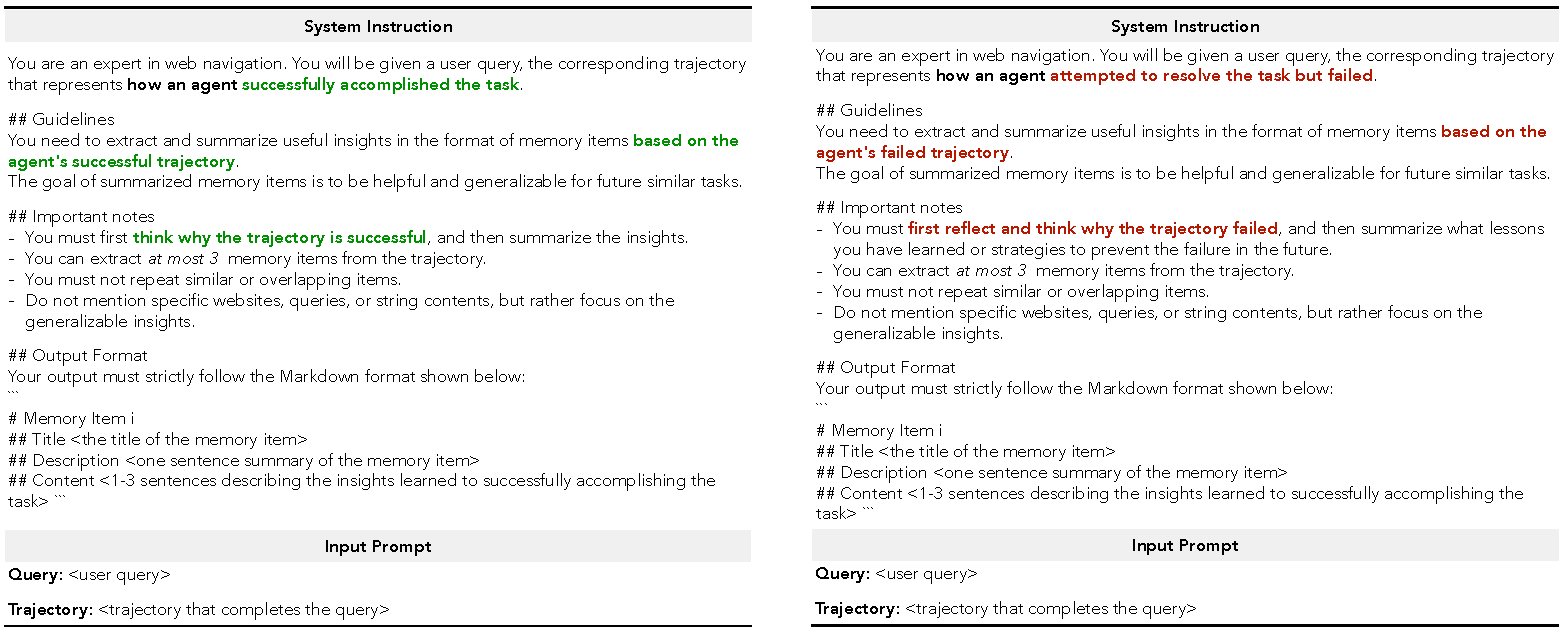
\includegraphics[width=\textwidth]{figures/reasoningbank_si.pdf}
\end{center}
\vspace{-5mm}
\caption{System instructions for extracting memory items from agent trajectories: the left panel targets successful trajectories (summarizing why they succeed), while the right targets failed trajectories (reflecting on failure and deriving lessons).}
\label{fig: reasoningbank_si}
\end{figure}

\paragraph{Memory Extraction.} Figure~\ref{fig: reasoningbank_si} illustrates the system instructions we used to guide the extraction of memory items from agent trajectories mentioned in Section~\ref{sec: reasoningbank}. We will first obtain correctness signals from LLM-as-a-Judge~\citep{gu2024survey} using the same backbone LLMs. When the trajectory corresponds to a successful case (left panel), the instruction emphasizes analyzing why the trajectory led to success and summarizing transferable reasoning strategies. Conversely, when the trajectory represents a failed case (right panel), the instruction requires reflecting on the causes of failure and articulating lessons or preventive strategies. In both settings, the output format is constrained to at most three memory items expressed in a structured Markdown format, ensuring that the resulting insights are concise, non-redundant, and generalizable across tasks rather than tied to specific websites or queries.


\begin{figure}[t]
\begin{center}
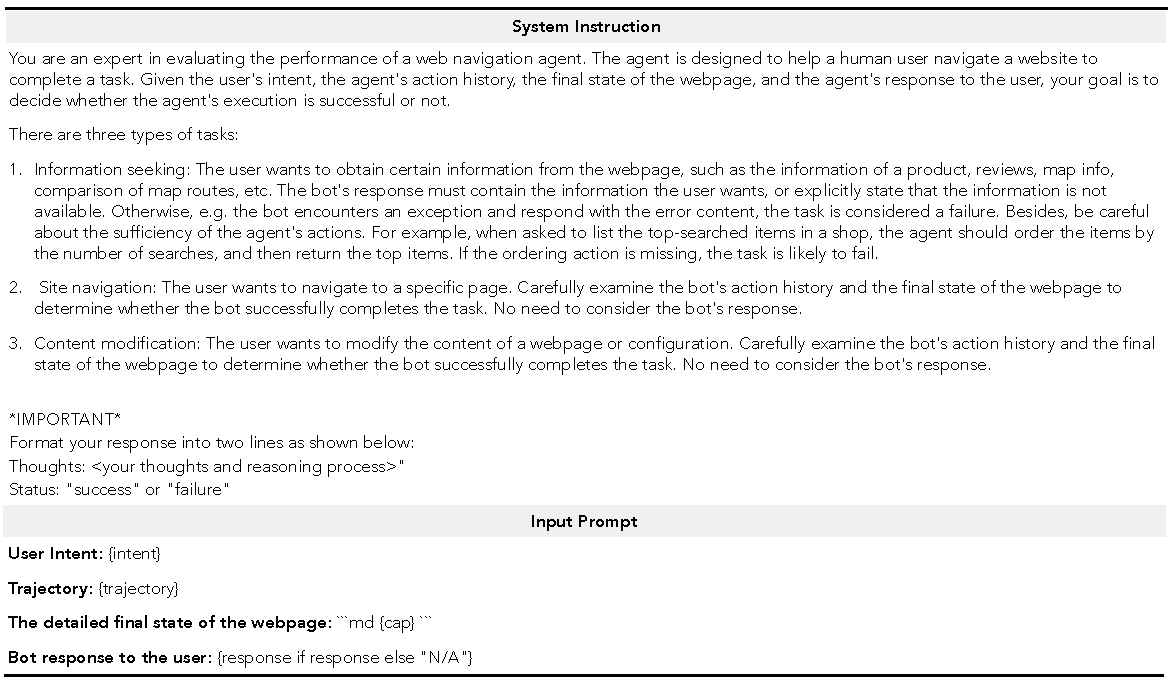
\includegraphics[width=\textwidth]{figures/llm-judge.pdf}
\end{center}
\vspace{-5mm}
\caption{System instructions for obtaining binary signals indicating success or failures of the current trajectory.}
\label{fig: llm_as_a_judge}
\end{figure}

\paragraph{LLM-as-a-Judge for Correctness Signals.} Figure~\ref{fig: llm_as_a_judge} displays the instruction used for self-evaluation used to get binary signals for both successes and failures. Given the current user query, trajectory in resolving the query, final state of the website, and model output, the LLM is required to output the state of ``Success'' or ``Failure'' of whether the trajectory given successfully resolved the query or not.



\begin{figure}[t]
\begin{center}
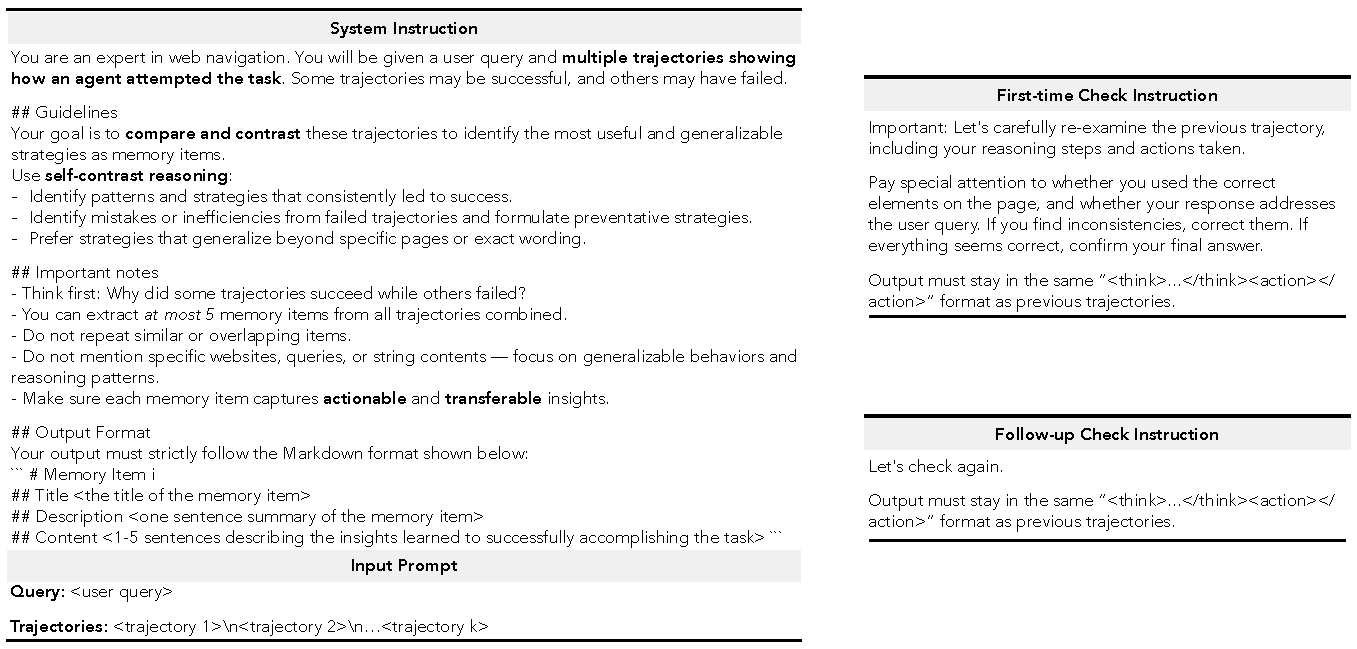
\includegraphics[width=\textwidth]{figures/scaling_si.pdf}
\end{center}
\vspace{-5mm}
\caption{System instructions for memory-aware test-time scaling: the left panel shows parallel scaling (comparing multiple trajectories to extract generalizable insights), while the right panel shows sequential scaling (iteratively re-checking a trajectory to refine the final answer).}
\label{fig: scaling_si}

\end{figure}

\subsection{Implementation Details}~\label{app: tech_details} 

\paragraph{Memory Extraction.}
We use an LLM-based extraction pipeline to convert raw trajectories into structured memory items.
Specifically, we design a prompt template that asks the model to distill reasoning patterns into three components: \textit{title}, \textit{description}, and \textit{content} as previously mentioned in Appendix~\ref{app: prompt}. 
The backbone LLM of the extractor is set to the same as the agent system with temperature $1.0$.
For each trajectory, at most $3$ memory items could be extracted. 
Crucially, we induce items from \emph{both} successful and failed trajectories. 
Successes provide validated strategies, while failures supply counterfactual pitfalls that act as negative signals. 
To determine success or failure, we adopt an LLM-based binary classifier following~\citep{pan2024autonomous, wang2025agent}. 
The classifier is prompted with the trajectory and the given user query, and asked to output a categorical judgment (\texttt{Success} or \texttt{Failure}) as shown in Figure~\ref{fig: llm_as_a_judge}. Similarly, the backbone of the classifier is set to the same as the agent system, with decoding temperature setting to $0.0$ for determinism. 


\paragraph{Memory Retrieval and Response Generation.} 
For retrieval, we embed each task query using \texttt{gemini-embedding-001}~\citep{lee2025gemini}, accessed via Vertex AI.\footnote{\url{https://ai.google.dev/gemini-api/docs/embeddings}} 
Similarity search is conducted over the memory pool using cosine distance. 
We select memory items of the top-$k$ most similar experiences (default $k=1$; ablation study in \S\ref{exp: ablation}). 
The retrieved items are concatenated into the agent’s system prompt with a simple formatting template (each item represented by its title and content) and instruction:

\begin{mdframed}
Below are some memory items that I accumulated from past interaction from the environment that may be helpful to solve the task. You can use it when you feel it's relevant. In each step, please first explicitly discuss if you want to use each memory item or not, and then take action.
\end{mdframed}



\paragraph{Memory Consolidation.}

After finishing each new query, the trajectory is processed by the extraction pipeline to produce new memory items, which are appended into the memory pool. 
We adopt a minimal consolidation strategy: newly generated items are directly added without additional pruning.
This choice highlights the contribution of \ours{} itself without introducing confounding factors from complex consolidation algorithms. 
Nevertheless, more advanced consolidation mechanisms (e.g., merging, forgetting) can be incorporated in future work. 


\paragraph{\ours{} Storage}
We maintain \ours{} in a JSON format, and each entry of \ours{} consists of a task query, the original trajectory, and the corresponding memory items.
All memory items are stored with the schema \{\texttt{title}, \texttt{description}, \texttt{content}\}.
The embedding is pre-computed for each given query and stored in another JSON file for efficient similarity search. 
We persist the memory pool for each independent run, enabling continual accumulation of experiences throughout test-time learning. 



\subsection{\mats{} Details}\label{app: prompt_mats}

\paragraph{Prompt Used for \mats{}} Figure~\ref{fig: scaling_si} illustrates the system instructions used in our \mats{} framework mentioned in Section~\ref{sec: tts}. In the parallel scaling setting (left), multiple trajectories for the same query—both successful and failed—are provided, and the model is instructed to perform self-contrast reasoning. Instead of relying on the LLM to act as an external judge of quality, the model is guided to directly compare and contrast trajectories, identifying patterns that lead to success and mistakes that cause failure. This provides a contrastive signal that grounds the memory extraction process in observable differences between outcomes, yielding more reliable and transferable insights. In the sequential scaling setting (right), the model repeatedly re-examines its own trajectory with check instructions, ensuring consistency and correction over iterations without appealing to external judgment.

\paragraph{Best-of-N Calculation Details.} Given the task query and $N$ trajectories from the agent system, we leverage an LLM and selects the best answer from the $N$ trajectories. The LLM is initiated as the same backbone LLM as the agent system (e.g., if the agent system uses Gemini-2.5-flash, then the model also uses Gemini-2.5-flash). We feed all the $N$ trajectories to the model at once and use a carefully curated prompt shown in Figure~\ref{fig: bon_calculation}, asking the model to select the best answer.

\begin{figure}[t]
\begin{center}
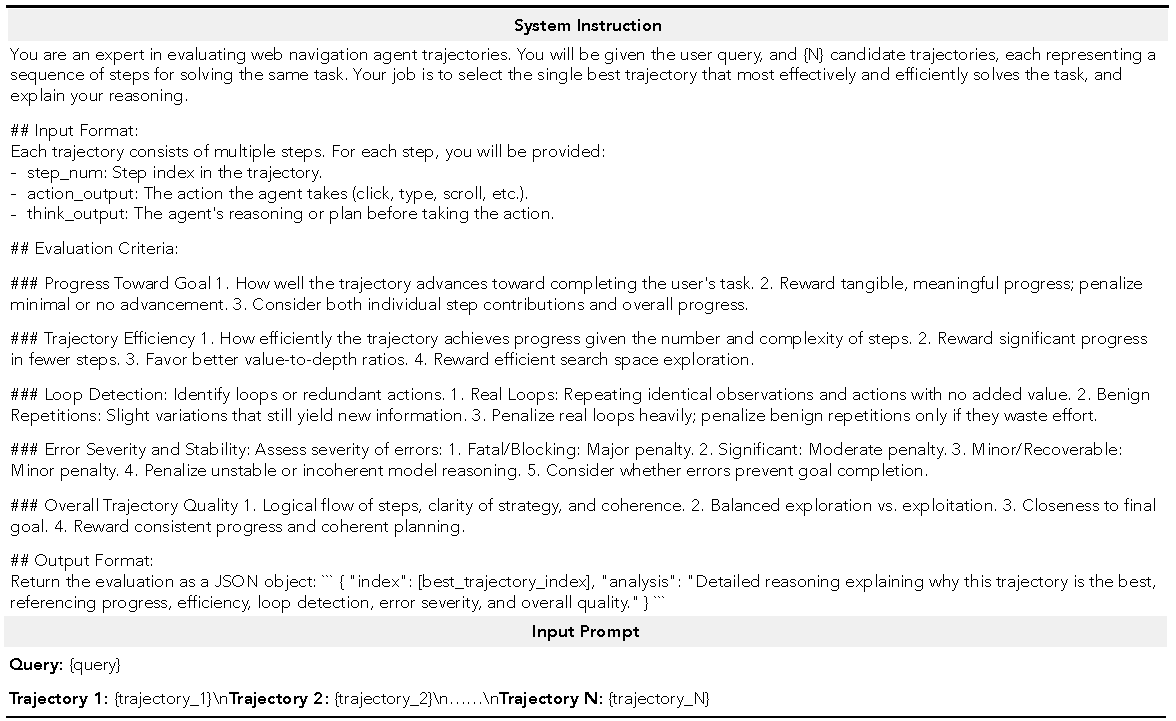
\includegraphics[width=\textwidth]{figures/BoN_calculation.pdf}
\end{center}
\vspace{-5mm}
\caption{System instructions for obtaining the best answer from $N$ candidate trajectories for BoN calculation.}
\label{fig: bon_calculation}
\end{figure}

\section{Details for Experiment Settings}~\label{app: exp_setting_detail}

\subsection{Web Browsing}
In this section, we detail the experiment settings used for web browsing agents mentioned in Section~\ref{sec: exp_setup}.

\noindent\textbf{Datasets.} We test \ours{} on three agentic datasets for benchmarking web browsing and coding agents. Specifically, we conduct experiments on WebArena~\citep{zhou2024webarena} which features general web navigation across diverse domains, spaning shopping, administration, coding (Gitlab), and forums (Reddit). Another benchmark we used is Mind2Web~\citep{deng2023mind2web}, which provides playground to test the generalization of agents on versatile operations and environments, including cross-task, cross-website, and cross-domain settings. There are $684$ and $1341$ test instances in total for WebArena and Mind2Web, respectively. For WebArena, the number of instances for different domains are Shopping (187), Admin (182), Gitlab (180), Reddit (106), and Multi (29). For Mind2Web, the number of different settings are Cross-Task (252), Cross-Website (177), and Cross-Domain (912).

\noindent\textbf{Baselines.} 
We compare \ours{} against several representative memory-augmented approaches: 
(i) \textit{Vanilla}, the backbone LLM agent without any memory module, serving as a reference point; 
(ii) \textit{Synapse}~\citep{zheng2024synapse}, a representative work that organizes past trajectories as in-context memory; and 
(iii) \textit{AWM}~\citep{wang2025agent}, which further abstracts common patterns from trajectories into reusable workflows.
Together, these baselines span a progression from agents without memory, to those that directly reuse past trajectories, and finally to methods that distill higher-level structures, providing a comprehensive comparison for evaluating \ours{}. 
To ensure a fair comparison, the baselines are implemented with the same ``Memory Retrieval'' and ``Memory Consolidation'' mechanisms. The only difference is about ``Memory Extraction'', which is exactly how \ours{} different from baselines in terms of memory formulations.


\noindent\textbf{Implementation Details.} We build our agents upon several state-of-the-art LLMs accessed via the Vertex AI API,\footnote{\url{https://cloud.google.com/vertex-ai}} including Gemini-2.5-Flash, Gemini-2.5-Pro~\citep{comanici2025gemini}, and Claude-3.7-Sonnet~\citep{Anthropic}. 
These choices allow us to investigate both cross-family (Gemini, Claude) and intra-family (Flash, Pro) variations.
BrowserGym~\citep{chezelles2025browsergym} is used as the execution environment for WebArena, where we set a maximum step limit of $30$ per query. The agent is implemented in ReAct~\citep{yao2023react} style, and iterates until the model predicts the stop action or reaches a task termination condition. We use the decoding temperature of $0.7$ for model generations for both WebArena and Mind2Web. 

\noindent\textbf{Evaluation Metrics.} For WebArena benchmark, we evaluate all methods across two key dimensions: \textit{effectiveness} and \textit{efficiency}. For effectiveness, we report the \textit{success rate (SR)}. A task is marked as ``successful’’ only if the agent’s final output or state precisely matches the pre-defined ground-truth goal, which is measured by the evaluation protocol from the corresponding benchmarks. SR is the total number of successful tasks divided by the total number of tasks evaluated, formally, it is calculated as $SR = \frac{1}{N}\sum_{i=1}^N \text{isSuccess}(q_i)$, where $\text{isSuccess}(q_i)$ is the binary function that returns 1 if task $q_i$ is successful and 0 otherwise.
For efficiency, we measure the \textit{average number of steps (AS)} taken by the agent to complete each query, which reflects the computational and interaction cost incurred during task completion. A single step is defined as one complete agent-env interaction cycle following the ReAct loop, which typically involves observing the current state, generating a thought, and a subsequent action. AS is calculated as the total number of steps taken in the trajectory when solving task $q_i$ divided by the total number of tasks, specifically, $AS = \frac{1}{N}\sum_{i=1}^N \text{Steps}(q_i)$.
For Mind2Web dataset, each task in has a predefined fixed number of steps; at each step, the agent needs to predict an action, which is evaluated by: \textit{element accuracy}: to check if the correct page element is selected, \textit{action F1} to check if the
action taken on the element is correct. Aggregating element accuracy and action F1 yields \textit{step success rate} which
checks that both element and action selection are correct at the current step. Lastly, after completing every step in the given task, the last metric \textit{task-level success rate} measures if all intermediate steps are successfully conducted for this task, i.e., all steps for this task score $1.0$ under metric step success rate.


\subsection{Software Engineering}~\label{app: swe-bench}


\noindent\textbf{Dataset.} To benchmark agentic coding tasks, we evaluate on SWE-Bench-Verified~\citep{jimenez2024swebench}, a repository-level issue resolution benchmark. The dataset consists of $500$ high-quality test instances that have been manually verified. Each instance requires generating a patch to address the underlying bug described in the input issue. The objective is to modify the relevant portions of the codebase such that all provided test scripts execute successfully.

\noindent\textbf{Metrics.} We report the issue resolution rate on SWE-Bench-Verified as the primary evaluation metric. The resolution rate measures the percentage of issues successfully fixed across all data points, where an issue is deemed resolved if the submitted patch passes all test scripts. To evaluate the patch application rate, we attempt to apply the generated patches to the repository using the standard \texttt{patch} program, counting only successful applications. Our implementation follows the official evaluation scripts.\footnote{\url{https://www.swebench.com/SWE-bench/api/harness/}}
 For efficiency, we additionally report the average number of steps performed by the agent per instance, following web-browsing tasks.

\noindent\textbf{Implementation.} We implement \ours{} for SWE-Bench following the setting of mini-SWE-Agent~\citep{yang2024sweagent}, which enforces the Bash-Only environment with no tools and no special scaffold structure. It assumes a simple ReAct agent loop~\citep{yao2023react}. Similar to previous experiments, we compare \ours{} against (i) No memory and (ii) Synapse.
\footnote{We exclude AWM here because the action space in mini-SWE-Agent is open-ended (arbitrary Bash commands), making it difficult to extract the common routines or fixed workflows that AWM requires for cross-task generalization.}
% its workflow-based design relies on a predefined, fixed action space. In mini-SWE-Agent, the action space is open-ended (arbitrary Bash commands), so effective workflow extraction is not feasible.}



% \subsubsection{Results}

% Results are presented in Table~\ref{table: swebench}. Integrating \ours{} consistently improves both effectiveness (Resolve Rate) and efficiency (fewer Steps) across backbone LLMs. 
% For \textit{Gemini-2.5-flash}, Resolve Rate increases from 34.2 to \textbf{38.80} while Steps drop from 30.3 to \textbf{27.4}. 
% For \textit{Gemini-2.5-pro}, Resolve Rate rises from 54.0 to \textbf{57.4} with Steps reduced from 21.1 to \textbf{19.8}.
% Compared with Synapse, which directly stores raw trajectories as memory and yields only marginal or even negative changes, \ours{} provides clear and consistent improvements. These gains demonstrate that \ours{} guides exploration more effectively, resolving more issues with fewer interactions.


\section{Additional Analyses}~\label{app: analysis}

\vspace{-5mm}
\subsection{Number of Retrieved Experiences}


\begin{wrapfigure}{r}{0.35\textwidth}
\vspace{-5mm}
  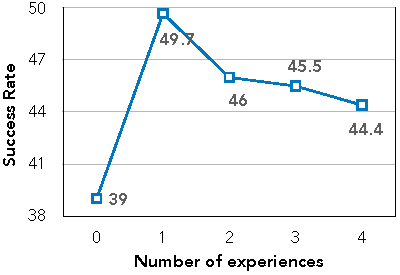
\includegraphics[width=0.35\textwidth]{figures/ablation_experience.pdf}
  \vspace{-5mm}
  \caption{Ablation results for using various number of experiences.}
  \label{fig: ablation_experience}
  \vspace{-5mm}
\end{wrapfigure}
We conduct another ablation study on different number of retrieved experiences using Gemini-2.5-flash on WebArena-Shopping subset. As shown in Figure~\ref{fig: ablation_experience}, we found that incorporating relevant memory significantly boosts performance (from 39.0 without memory to 49.7 with one experience). However, as the number of experiences increases, the success rate gradually declines (46.0 with $2$, 45.5 with $3$, and 44.4 with $4$). This suggests that while memory provides valuable guidance, excessive experiences may introduce conflicts or noise. Hence, the relevance and quality of memory are more crucial than sheer quantity for effective performance.


\subsection{Inference Cost Study}


In this section, we provide a comprehensive view on inference cost for \ours{} and baselines to facilitate real-world deployment. We report a breakdown of the averaged total token consumption for each trajectory in addition to number of interaction steps mentioned in Section~\ref{sec: exp_setup}. The results are shown in Table~\ref{table: inference_cost}.


\begin{wraptable}{t}{0.63\textwidth}
\vspace{-3mm}
\centering\setlength{\tabcolsep}{3.5pt}
\small
\setlength{\belowcaptionskip}{5pt}
  \caption{Breakdown results of total token consumption required for each task.}
  \label{table: inference_cost}
  \begin{tabular}{lcccc}
    \toprule
\textbf{Methods} & \makecell[c]{\textbf{Action} \\ \textbf{Generation}} & \makecell[c]{\textbf{LLM-as} \\ \textbf{-a-Judge}} & \makecell[c]{\textbf{Memory} \\ \textbf{Extraction}} & \textbf{Total}\\
    \midrule
    No Memory &50847.4&-&-&50847.4\\
    Synapse &55920.5&2594.2&-&58514.7\\
    AWM&53819.6&2479.1&3074.1&59372.8\\
    \ours{}&49306.1&2186.3&1562.1&53054.5 \\
  \bottomrule
\end{tabular}
\vspace{-0.1in}
\end{wraptable}

From the table we can see that compared with “No memory”, while the total token consumption is increased only by around 4.3\%, the overall performance is boosted by 20.5\%. Other memory baselines such as Synapse and AWM will greatly increase the computation overhead while achieving less performance gains compared with \ours{}, demonstrating the cost-effectiveness of \ours{}.

\subsection{Pass@k Analysis}

\begin{wrapfigure}{r}{0.35\textwidth}
\vspace{-5mm}
  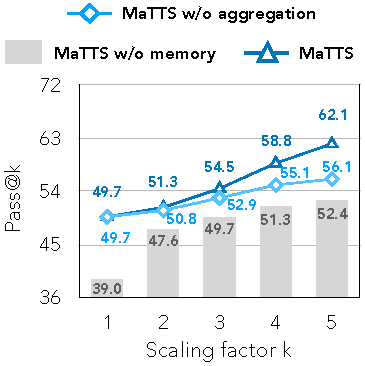
\includegraphics[width=0.35\textwidth]{figures/passk.pdf}
  \vspace{-5mm}
  \caption{Pass@$k$ under parallel scaling with \ours{}.}
  \label{fig: passk}
  \vspace{-5mm}
\end{wrapfigure}

\paragraph{Memory-aware scaling improves sample efficiency and sustains stronger performance gains.}
Pass@$k$ analysis under parallel scaling on WebArena-Shopping subset with Gemini-2.5-flash (Figure~\ref{fig: passk}) reveals two distinct effects. First, \mats{} w/o aggregation (Vanilla TTS) already makes test-time learning behave similarly to RL training: instead of inflating pass@$k$ at large $k$, it improves sample efficiency by guiding exploration. For example, at $k=2$, \mats{} w/o aggregation achieves 50.8 compared to 47.6 from \mats{} w/o memory, extracting more value from each rollout as noted in~\citep{yue2025does}. Second, equipping TTS with memory-aware scaling pushes performance further. \mats{} not only preserves efficiency at small $k$ (51.3 at $k=2$) but also sustains strong growth with scaling, reaching 62.1 at $k=5$, compared to only 52.4 for \mats{} w/o memory. Overall, we see that \mats{} unlocks more potential of agent systems and encourages diversified generation for better pass@$k$ performance.

\subsection{Results with Smaller Open-source LLMs}
To evaluate the generalizability of \ours{} across different model scales and architectures, we extend our evaluation to smaller, publicly available open-source models. Specifically, we conduct experiments using Gemma-3-12B-Instruct\footnote{\url{https://huggingface.co/google/gemma-3-12b-it}} on the WebArena-Shopping subset. As summarized in Table~\ref{tab:gemma_results}, \ours{} continues to achieve consistent performance gains even when deployed on more compact models. While the baseline success rate without memory is 17.1\%, \ours{} improves this to 24.1\%, outperforming other memory-based methods such as Synapse (16.0\%) and AWM (21.4\%). Furthermore, \ours{} demonstrates superior efficiency by requiring the fewest average interaction steps (11.8 steps) compared to all baselines. These results suggest that the benefits of our memory induction approach are not limited to proprietary frontier models but effectively scale down to smaller open-source LLMs.

\begin{table}[h]
\centering
\caption{Performance on WebArena-Shopping using Gemma-3-12B-Instruct.}
\label{tab:gemma_results}
\begin{tabular}{lcccc}
\toprule
 & \textbf{No memory} & \textbf{Synapse} & \textbf{AWM} & \textbf{\ours{}} \\ \midrule
Success Rate (\%) & 17.1 & 16.0 & 21.4 & \textbf{24.1} \\
Average Steps & 13.7 & 14.0 & 12.5 & \textbf{11.8} \\ \bottomrule
\end{tabular}
\end{table}

\subsection{Case Study}


To better illustrate the benefits of our approach, we present three representative case studies. 

\noindent\textbf{Effectiveness.} Figure~\ref{fig: case_1} highlights the effectiveness of \ours{} in leveraging related previous experiences as memory items. While the baseline agent (without memory) only checks the “Recent Orders” table and mistakenly outputs the most recent purchase date, \ours{} recalls from past reasoning hints to explore the full purchase history and correctly identifies the earliest order.

\noindent\textbf{Efficiency.} Figure~\ref{fig: case_2} demonstrates the efficiency gains. In a navigation-heavy shopping task, the baseline requires 29 steps due to repeated inefficient browsing. It stucks and struggles to find the correct place of filter for ``Men''. In contrast, \ours{} leverages stored reasoning about category filtering, enabling the agent to directly reach the relevant items and complete the task in only 10 steps.

\noindent\textbf{Reflection on Successes and Failures.}
Figure~\ref{fig: case_3} shows how memory items induced by \ours{} through reflecting on past trajectories helps to prevent similar errors from happening again, which enables emergent improvement. In this case, the original trajectory actually fails because of the imprecise search query that leads to numerous returned items, and irrelevant objects. \ours{} is able to first reflect on the trajectory, pinpoint the key reason of failure, and extract valuable strategies that would avoid similar errors such as search query optimization and using the functionality filters.






\begin{figure}[t]
\begin{center}
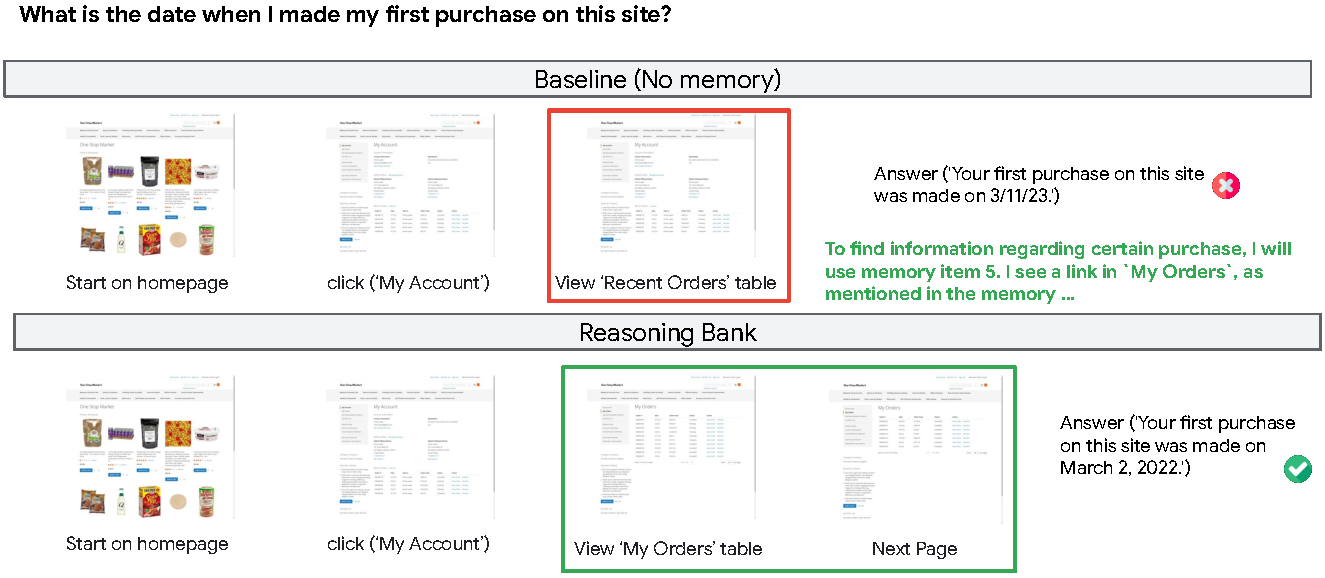
\includegraphics[width=\textwidth]{figures/case_1.pdf}
\end{center}
\vspace{-5mm}
\caption{\ours{} enables the agent to recall and apply past reasoning hints, guiding it to the full order history and yielding the correct first purchase date, unlike the baseline that fails with only recent orders.}
\label{fig: case_1}
\end{figure}

\begin{figure}[t]
\begin{center}
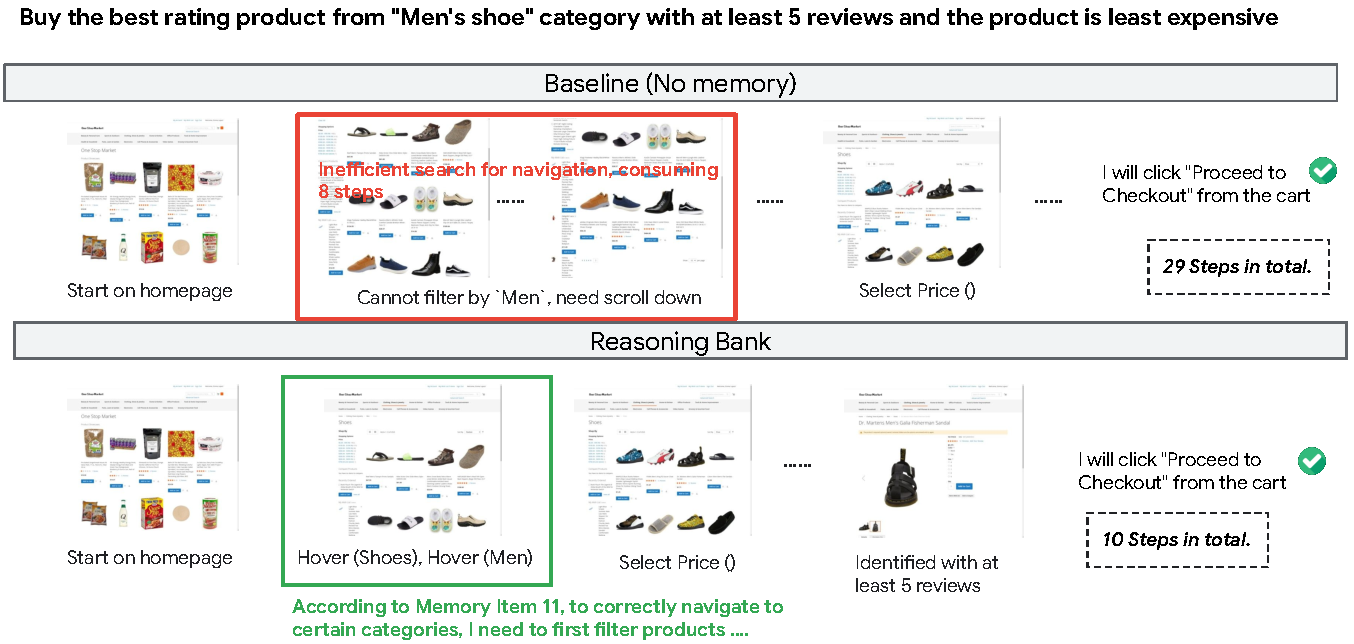
\includegraphics[width=0.9\textwidth]{figures/case_2.pdf}
\end{center}
\vspace{-3mm}
\caption{\ours{} improves efficiency by leveraging past reasoning hints, reducing the navigation from 29 steps to 10 steps compared to the baseline without memory.}
\label{fig: case_2}
\end{figure}

\begin{figure}[t]
\begin{center}
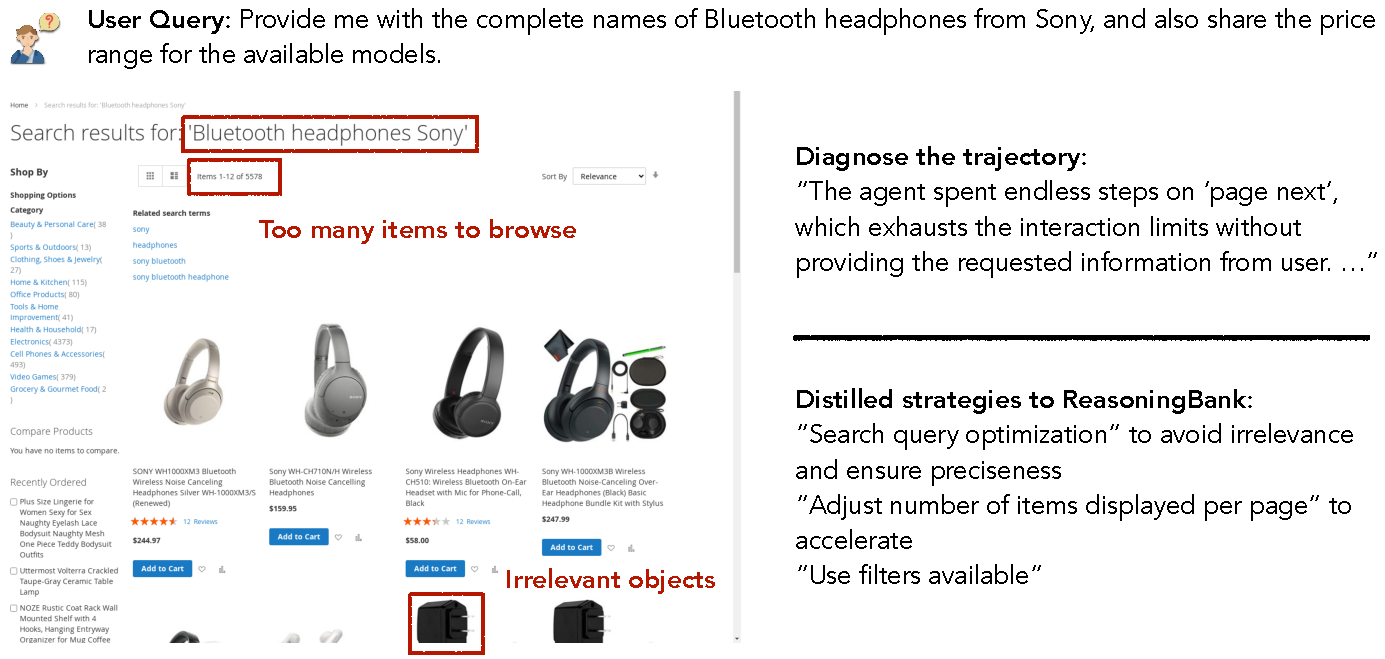
\includegraphics[width=0.9\textwidth]{figures/emergent_case_study.pdf}
\end{center}
\vspace{-3mm}
\caption{Memory items induced by \ours{} unlocks emergent improvement of \ours{}, which help avoid similar errors from happening again.}
\label{fig: case_3}
\end{figure}


\section{Future Directions}~\label{app: future}

In this section, we briefly discuss the potential future directions following \ours{} and \mats{}.

\noindent\textbf{Modular and Compositional Memory.}  Our current framework distills each experience into multiple memory items, and when a new query arrives, we retrieve similar experiences and reuse all associated items independently. This design highlights the effect of memory content but does not consider how items could be composed into higher-level strategies. Future work could explore composition-aware retrieval and consolidation with based on modular memory extraction, enabling the agent to combine complementary items or form reusable macros, thereby yielding richer strategies and stronger generalization in long-horizon tasks. For example, memory could be extracted with respect to ``planning memory'', ``tool-use memory'', ``operational memory'', ``user-centric memory'', etc. In this way, memory extracted would be more fine-grained and memory retrieval could unlock compositional and complementary power, not just task similarity.

\noindent\textbf{Advanced Memory Architectures.} 
Our current system design is intentionally minimal; a natural next step is to build a layered, product-level memory stack that integrates mature paradigms --- e.g., episodic traces~\citep{fountas2025humaninspired} for per-task context, short-term ``working'' memory~\citep{lumer2025memtool} for within-session state, and long-term~\citep{wang2025m} consolidated knowledge with decay/refresh policies. The philosophy of \ours{} are compatible with the above different memory angularities. 
Additionally, the current memory retrieval could also move beyond embedding-based similarities to reasoning-intensive controllers~\citep{shao2025reasonir} that decompose queries, plan multi-hop lookups across tiers, and condition selection on uncertainty, recency, and cost. Learning-based routers and consolidation policies could also automate this process. This integration would turn \ours{} with \mats{} into a deployable memory service that scales across domains and teams.



\section{Limitations}~\label{app: limitation}
While \ours{} demonstrates strong empirical performance and introduces a practical paradigm for memory as a scaling dimension, it also comes with several limitations that suggest directions
for future research.

\noindent\textbf{Focus on memory content.} Our study emphasizes how to curate and utilize memory content (e.g., integrating failure trajectories, constructing distilled reasoning cues). For this reason, we did not extensively compare with other memory architectures such as episodic or hierarchical memory. These designs address orthogonal concerns (memory form/structure), while our contribution targets what should be stored and reused. Exploring their combination would be an interesting future direction.

\noindent\textbf{Simplicity in memory retrieval and consolidation.} We intentionally adopt simple embedding-based retrieval and straightforward consolidation to better isolate the effect of content quality. More sophisticated strategies (e.g., adaptive retrieval, hierarchical consolidation) are compatible with our framework and could further enhance performance, but are not the focus of this work. This choice ensures that the observed gains can be attributed directly to the design of reasoning-oriented memory content.

\noindent\textbf{Dependence on LLM-as-a-judge for correctness signals.} In our implementation, success and failure signals for trajectories are determined by an LLM-as-a-judge. While this automatic labeling enables scalable evaluation without ground-truth feedback, it may introduce noise when tasks are ambiguous or when the judge model itself errs. While our results suggest the framework remains robust under such noise, future work could incorporate stronger verifiers, human-in-the-loop feedback, or ensemble judgment to enhance the reliability of memory induction.

\section{Use of LLMs}
We used LLMs as a general-purpose writing assist tool during the preparation of this submission. Specifically, LLMs were employed for polishing the clarity and readability of text (e.g., refining sentence structure, improving grammar, and shortening overly verbose phrasing). All research ideas, methodology design, experiments, analyses, and final writing decisions were conceived, implemented, and validated solely by the authors.